% ***********************************************************
% ******************* PHYSICS HEADER ************************
% ***********************************************************
% Version 2
\documentclass[11pt]{article} 
\usepackage{amsmath} % AMS Math Package
\usepackage{amsthm} % Theorem Formatting
\usepackage{amssymb}	% Math symbols such as \mathbb
\usepackage{graphicx} % Allows for eps images
\usepackage{multicol} % Allows for multiple columns
\usepackage[dvips,letterpaper,margin=0.75in,bottom=0.5in]{geometry}
 % Sets margins and page size
\pagestyle{empty} % Removes page numbers
\makeatletter % Need for anything that contains an @ command 
\renewcommand{\maketitle} % Redefine maketitle to conserve space
{ \begingroup \vskip 10pt \begin{center} \large {\bf \@title}
	\vskip 10pt \large \@author \hskip 20pt \@date \end{center}
  \vskip 10pt \endgroup \setcounter{footnote}{0} }
\makeatother % End of region containing @ commands
\renewcommand{\labelenumi}{(\alph{enumi})} % Use letters for enumerate
% \DeclareMathOperator{\Sample}{Sample}
\let\vaccent=\v % rename builtin command \v{} to \vaccent{}
\renewcommand{\v}[1]{\ensuremath{\mathbf{#1}}} % for vectors
\newcommand{\gv}[1]{\ensuremath{\mbox{\boldmath$ #1 $}}} 
% for vectors of Greek letters
\newcommand{\uv}[1]{\ensuremath{\mathbf{\hat{#1}}}} % for unit vector
\newcommand{\abs}[1]{\left| #1 \right|} % for absolute value
\newcommand{\avg}[1]{\left< #1 \right>} % for average
\let\underdot=\d % rename builtin command \d{} to \underdot{}
\renewcommand{\d}[2]{\frac{d #1}{d #2}} % for derivatives
\newcommand{\dd}[2]{\frac{d^2 #1}{d #2^2}} % for double derivatives
\newcommand{\pd}[2]{\frac{\partial #1}{\partial #2}} 
% for partial derivatives
\newcommand{\pdd}[2]{\frac{\partial^2 #1}{\partial #2^2}} 
% for double partial derivatives
\newcommand{\pdc}[3]{\left( \frac{\partial #1}{\partial #2}
 \right)_{#3}} % for thermodynamic partial derivatives
\newcommand{\ket}[1]{\left| #1 \right>} % for Dirac bras
\newcommand{\bra}[1]{\left< #1 \right|} % for Dirac kets
\newcommand{\braket}[2]{\left< #1 \vphantom{#2} \right|
 \left. #2 \vphantom{#1} \right>} % for Dirac brackets
\newcommand{\matrixel}[3]{\left< #1 \vphantom{#2#3} \right|
 #2 \left| #3 \vphantom{#1#2} \right>} % for Dirac matrix elements
\newcommand{\grad}[1]{\gv{\nabla} #1} % for gradient
\let\divsymb=\div % rename builtin command \div to \divsymb
\renewcommand{\div}[1]{\gv{\nabla} \cdot #1} % for divergence
\newcommand{\curl}[1]{\gv{\nabla} \times #1} % for curl
\let\baraccent=\= % rename builtin command \= to \baraccent
\renewcommand{\=}[1]{\stackrel{#1}{=}} % for putting numbers above =
\newtheorem{prop}{Proposition}
\newtheorem{thm}{Theorem}[section]
\newtheorem{lem}[thm]{Lemma}
\theoremstyle{definition}
\newtheorem{dfn}{Definition}
\theoremstyle{remark}
\newtheorem*{rmk}{Remark}

% ***********************************************************
% ********************** END HEADER *************************
% ***********************************************************
\usepackage{cancel}
\usepackage{verbatim}
\usepackage{enumerate}
\usepackage{pdfpages}
\usepackage{graphicx}
\usepackage{amsmath}
\usepackage{appendix}
\title{Comp 350-Assignment 5}
\author{Ian Benlolo 260744397\\McGill University\\}
\begin{document}
\maketitle

\begin{enumerate}[1.]
\item
\textbf{Vandermonde Form}\\
We start by building the Vandermonde matrix A and the equality $Ac=y$.
$$
\begin{bmatrix}
1 & 1 & 1 & 1 \\
1 & 2 & 2^2 & 2^3\\
1 & 3 & 3^2 & 3^3\\
1 & 4 & 4^2 & 4^3
\end{bmatrix}
\begin{bmatrix}
c_0 \\c_1\\ c_2\\ c_3
\end{bmatrix}
=
\begin{bmatrix}
y_0 \\ y_1 \\y_2 \\y_3
\end{bmatrix}
=
\begin{bmatrix}
2\\0\\-10\\-34
\end{bmatrix}
$$
We solve this with GEPP.\\
$$
\begin{bmatrix}
1 & 1 & 1 & 1 & \vline & 2 \\
1 & 2 & 2^2 & 2^3 & \vline & 0\\
1 & 3 & 3^2 & 3^3 & \vline & -10\\
1 & 4 & 4^2 & 4^3 & \vline & -34
\end{bmatrix}
\xrightarrow[R_{2,3,4}-R_1]{ }
\begin{bmatrix}
1 & 1 & 1 & 1 & \vline&  2\\
0 & 1 & 3 & 7& \vline & -2\\
0 & 2 & 8 & 26& \vline & -12\\
0 & 3 & 15 & 63 & \vline & -36
\end{bmatrix}
\xrightarrow[R_{3}-2R_2]{ R_4-3R_2}
\begin{bmatrix}
1 & 1 & 1 & 1 & \vline&  2\\
0 & 1 & 3 & 7& \vline & -2\\
0 & 0 & 2 & 12 & \vline & -8\\
0 & 0 & 6 & 42 & \vline & -30
\end{bmatrix}
$$
$$
\xrightarrow[R_{4}-3R_3]{R_3/2 }
\begin{bmatrix}
1 & 1 & 1 & 1 & \vline&  2\\
0 & 1 & 3 & 7& \vline & -2\\
0 & 0 & 1 & 6 & \vline & -4\\
0 & 0 & 0 & 6 & \vline & -6
\end{bmatrix}
\xrightarrow[]{R_4/6}
\begin{bmatrix}
1 & 1 & 1 & 1 & \vline&  2\\
0 & 1 & 3 & 7& \vline & -2\\
0 & 0 & 1 & 6 & \vline & -4\\
0 & 0 & 0 & 1 & \vline & -1
\end{bmatrix}
$$
From this we get  $c_3=-1, c_2=2, c_1=-1, c_0=2$.\\
$\therefore p_3(x)=c_0+c_1x+c_2x^2+c_3x^3=2-x+2x^2-x^3$\\

\textbf{Lagrange Form}\\

$L_1(x)=\frac{(x-2)(x-3)(x-4)}{(1-2)(1-3)(1-4)}=-\frac{x^3}{6}+\frac{3x^2}{2}-\frac{13x}{3}+4, L_2(x)=\frac{(x-1)(x-3)(x-4)}{(2-1)(2-3)(2-4)}=\frac{1}{2}(x^3 - 8 x^2 + 19 x - 12) , L_3(x)=\frac{(x-1)(x-2)(x-4)}{(3-1)(3-2)(3-4)}=-\frac{x^3}{2} + \frac{7 x^2}{2} - 7 x + 4, L_4(x)=\frac{(x-1)(x-2)(x-3)}{(4-1)(4-2)(4-3)}=\frac{1}{6} (x^3 - 6 x^2 + 11 x - 6)$\\

Now,\\
$p_3(x)=2\times L_1(x)+0\times L_2(x)-10\times L_3(x)-34\times L_4(x)=\dots=-x^3+2x^2-x+2$\\


\textbf{Newton Form}
We start by calculating $a_{k's}$:\\
$a_0=2$\\ $a_1=f[x_0,x_1]=\frac{f[x_1]-f[x_0]}{x_1-x_0}=\frac{0-2}{2-1}=-2$\\
$f[x_1,x_2]=\frac{f[x_2]-f[x_1]}{x_2-x_1}=\frac{-10-0}{3-2}=-10$\\
$\therefore a_2=f[x_0,x_1,x_2]=\frac{f[x_1,x_2]-f[x_0,x_1]}{x_2-x_0}=\frac{-10-(-2)}{3-1}=-4$\\
$f[x_2,x_3]=\frac{f[x_3]-f[x_2]}{x_3-x_2}=\frac{-34-(-10)}{4-3}=-24$\\$f[x_1,x_2,x_3]=\frac{f[x_2,x_3]-f[x_1,x_2]}{x_3-x_1}=\frac{-24-(-10)}{4-2}=-7$\\
$\therefore a_3=f[x_0,x_1,x_2,x_3]=\frac{f[x_1,x_2,x_3]-f[x_0,x_1,x_2]}{x_3-x_0}=\frac{-7-(-4)}{4-1}=-1$\\

Now,\\
$$p_3(x)=a_0+a_1(x-x_0)+a_2(x-x_0)(x-x_1)+a_3(x-x_0)(x-x_1)(x-x_2)$$$$=2-2(x-1)-4(x-1)(x-2)-1(x-1)(x-2)(x-3)=\dots=-x^3+2x^2-x+2$$

\item 
	\begin{enumerate}[(a)]

\item
\begin{figure}[h!]
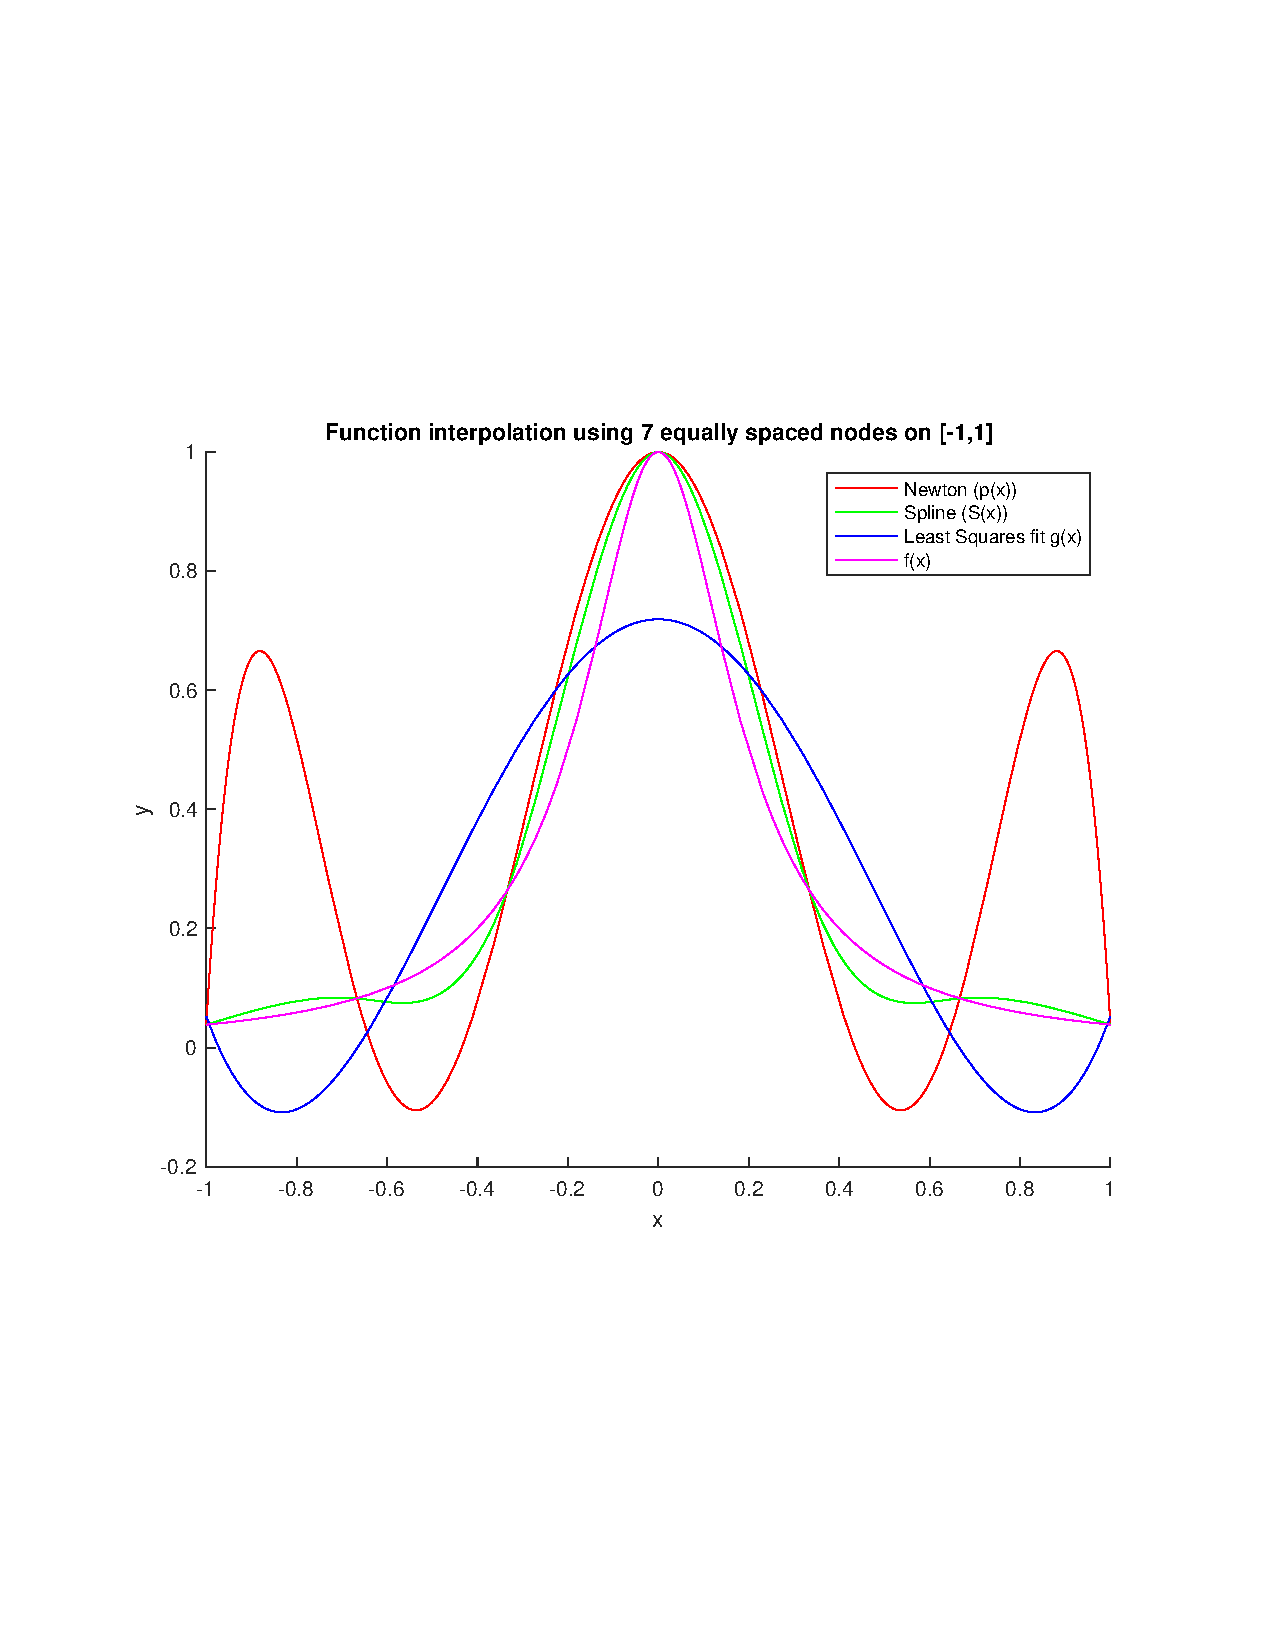
\includegraphics[width=\textwidth]{q2a.pdf}
\end{figure}

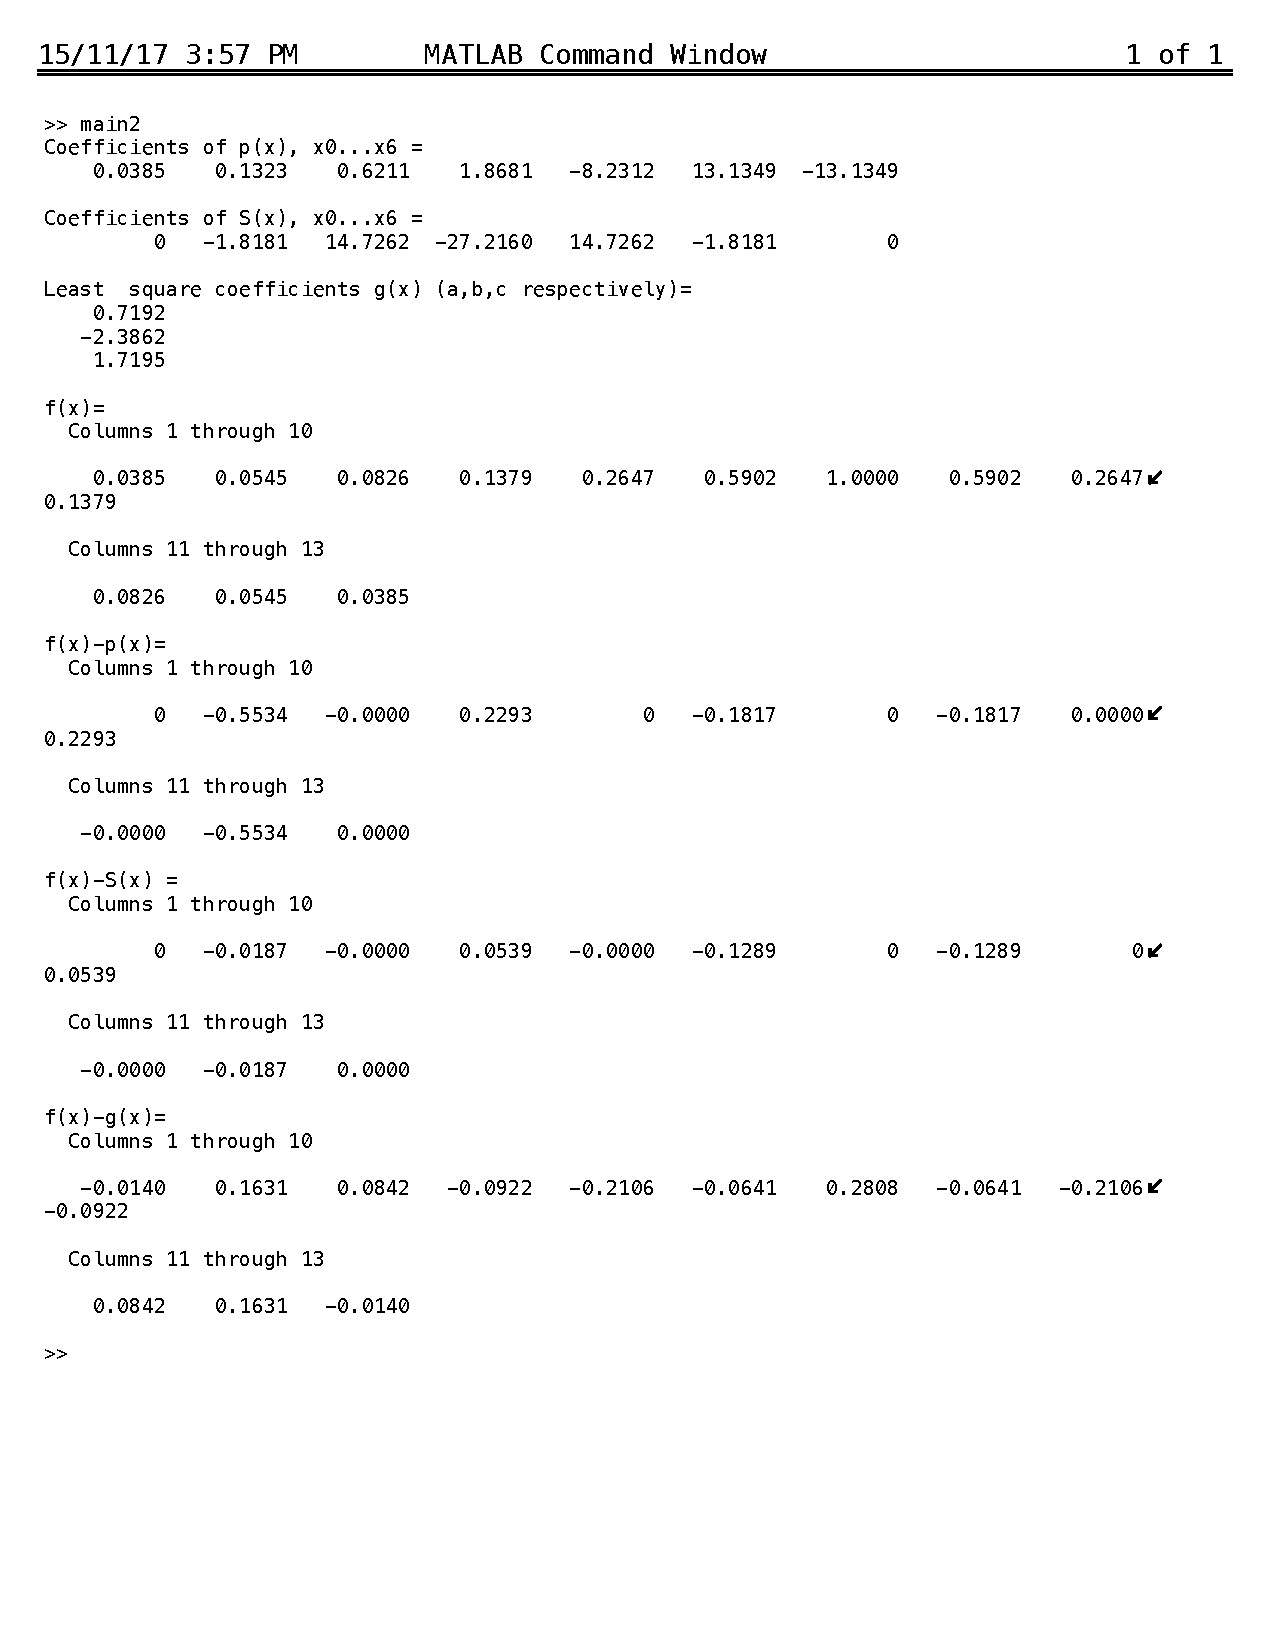
\includepdf[pages=-1]{q2avals.pdf}.


\newpage

\item.
\begin{figure}[hb!]
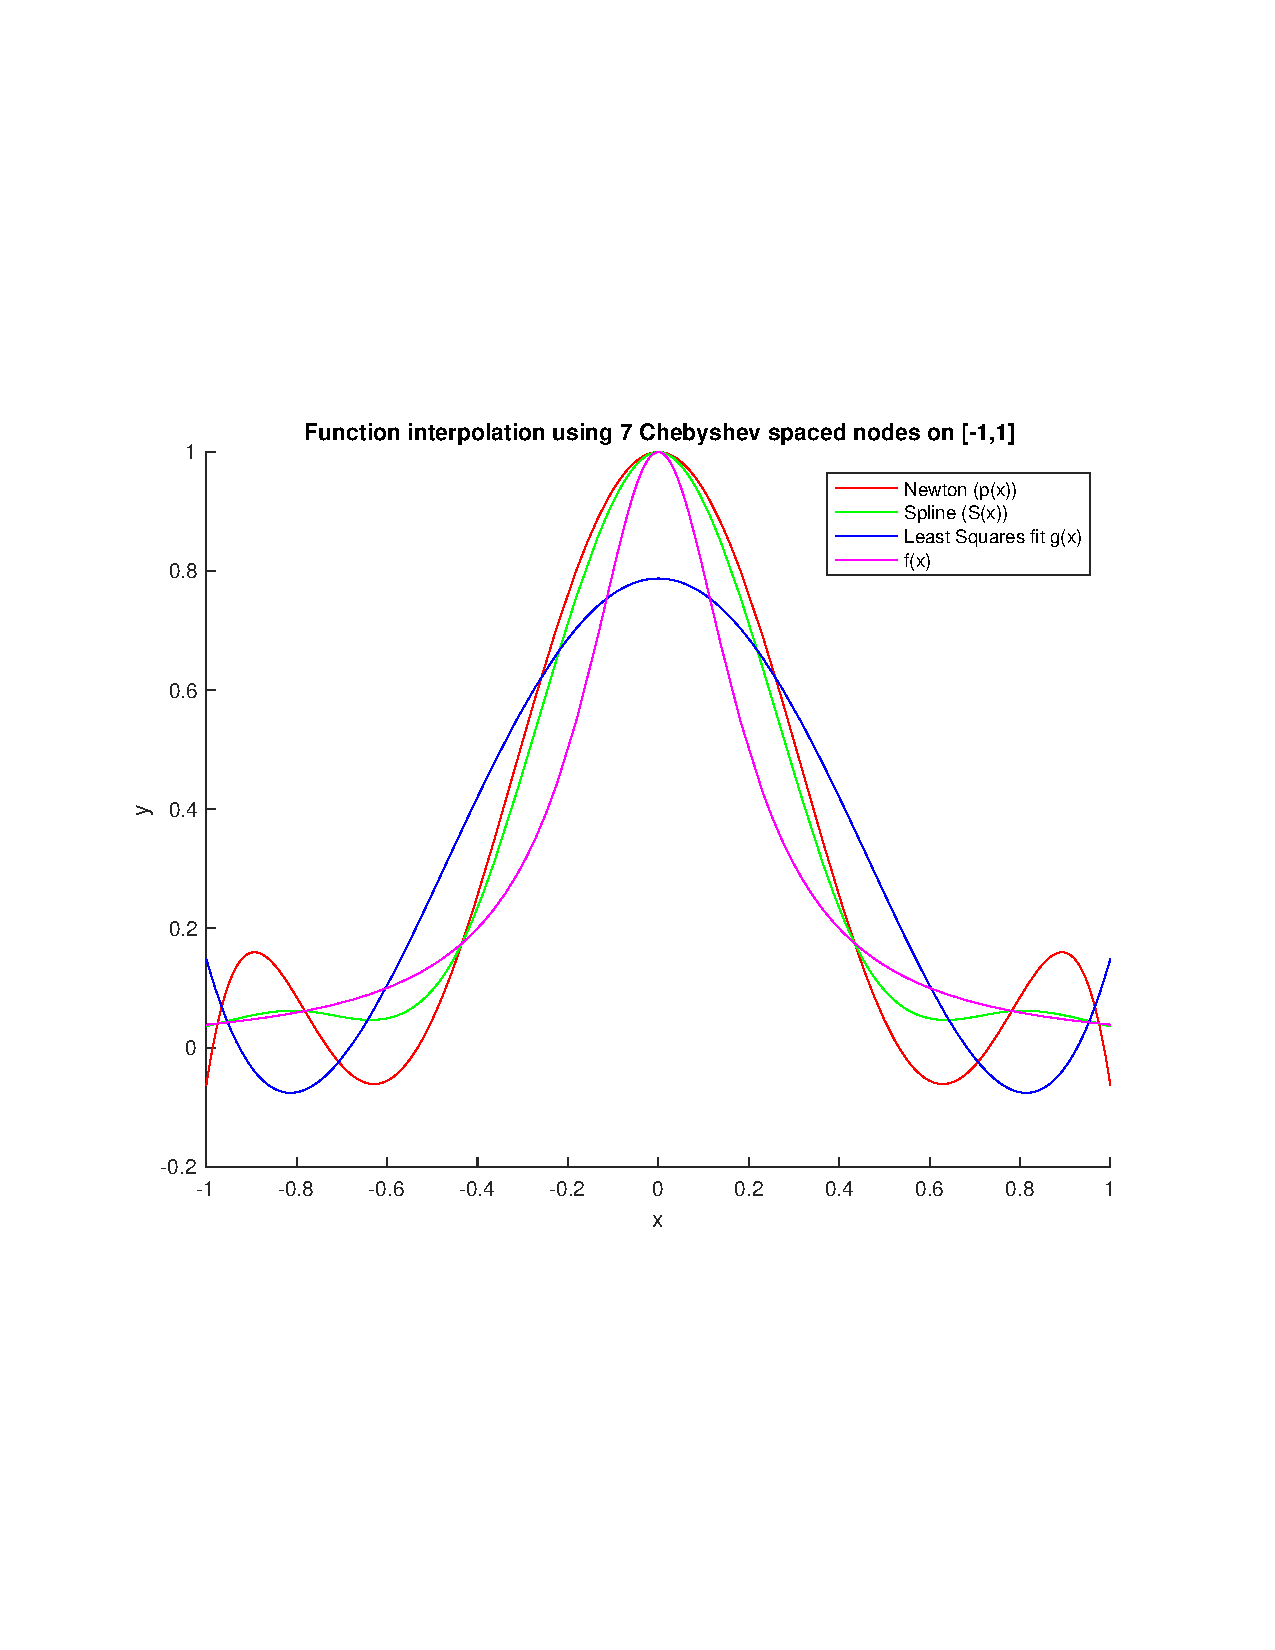
\includegraphics[width=\textwidth]{q2b.pdf}
\end{figure}

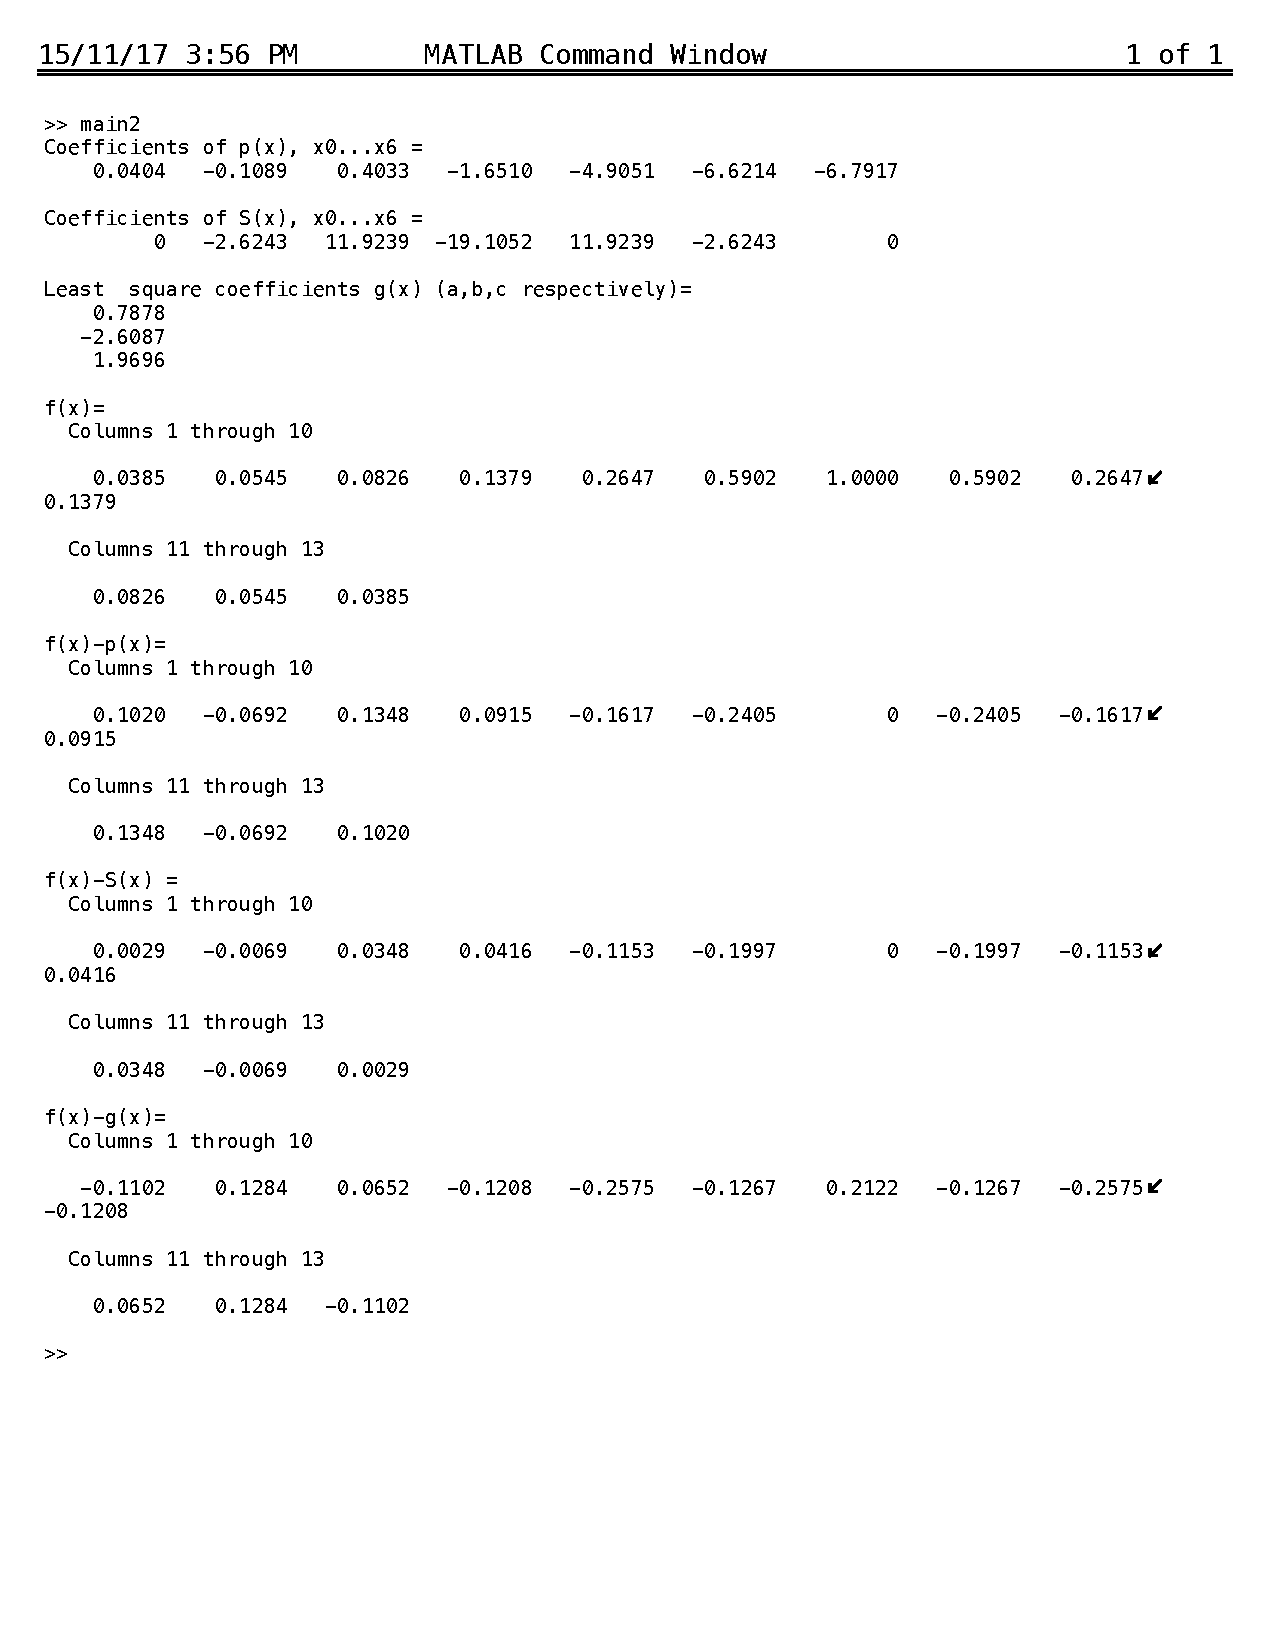
\includepdf[pages=-1]{q2bvals.pdf}

\newpage

\item The plots that used the Chebyshev nodes were closer to $f(x)$ since these nodes are better for interpolating for all methods. This is especially visible at both ends of the functions, though at the center (~x=0) the $7$ equally spaced nodes seem to interpolate the functions much better than the later. Furthermore, all three interpolations using the Chebyshev nodes are much more similar to each other as well. In general, the Chebyshev nodes form quite a good set of nodes for polynomial interpolation.\\

\end{enumerate}

\textbf{Matlab code.} Main functions included as .m file on mycourses\\
\begin{verbatim}
function y = newtonEval(x)
%coord=0for the 7 equally spaced, 1 for chebyshev
nodes= 0;
a = Newton(nodes);
n = length(a);

if nodes==0
    coord=linspace(-1,1,7);
elseif nodes==1 %for chebyshev
    for i=0:6
        coord(i+1)=cos((2*i+1)*pi/(2*6+2));
    end
end

y = a(n);

xi = coord(1,:);

for i=n-1: -1:1
    y = a(i) + y.*(x-xi(i));
end

----------------------------------
function a=Newton(nodes)
n=7;
if nodes==0
    xs=linspace(-1,1,7);
elseif nodes==1 %for chebyshev
    for i=0:6
        xs(i+1)=cos((2*i+1)*pi/(2*6+2));
    end
end
for i=1:n
    y(i)=f(xs(i));
end

for k=1:n-1
    a(k)=y(k);
    for i=k+1:n
        y(i)=(y(i)-y(k))/(xs(i)-xs(k));
    end
end
a(n)=y(n);

----------------------------------
function g=leastSquaresEval(x)
coord=0;
p=leastSquares(coord);
g=p(1)+p(2)*x.^2+p(3)*x.^4;
----------------------------------
function c=leastSquares(coord)
%coord=0 for 7 equally spaced nodes, 1 for chebyshev nodes
n=7;
if coord==0
    x=linspace(-1,1,7);
elseif coord==1 %for chebyshev
    for i=0:6
        x(i+1)=cos((2*i+1)*pi/(14));
    end
end
for i=1:7
    y(i)=f(x(i));
end
a=zeros(n,3);
for i=1:n
    a(i,1)=x(i)^0;
    a(i,2)=(x(i))^2;
    a(i,3)=(x(i))^4;
end

c=a\transpose(y);

----------------------------------
function z=calcZ(coords)

if coords==0
    x=linspace(-1,1,7);
elseif coords==1 %for chebyshev
    for i=0:6
        x(i+1)=cos((2*i+1)*pi/(14));
    end
    x=fliplr(x);
end
n=length(x);
for i=1:n
    y(i)=f(x(i));
end

for i=1:n-1
    h(i)=x(i+1)-x(i);
    b(i)=(y(i+1)-y(i))/h(i);
end

%forward elimination
u(2)=2*(h(1) + h(2));
v(2)=6*(b(2) - b(1));

for i=3:n-1
    u(i)=2*(h(i-1)+h(i)) - ((h(i-1))^2)/u(i-1);
    v(i)=6*(b(i)-b(i-1))-(h(i-1)*v(i-1))/u(i-1);
end

%back substitution
z(n)=0;
for i=n-1:-1:2
    z(i)=(v(i)-h(i)*z(i+1))/u(i);
end
z(1)=0;
----------------------------------

function S=cubicSpline(x)
coord=0;
if coord==0
    t=linspace(-1,1,7);
elseif coord==1 %for chebyshev
    for i=0:6
        t(i+1)=cos((2*i+1)*pi/(14));
    end
    t=fliplr(t);
end
n=length(t);
z=calcZ(coord);
for i=1:n
    y(i)=f(t(i));
end

for i=1:n-1
    if x<=t(i+1)
        break;
    end
end
h = t(i+1)-t(i);
B = -(h*z(i+1)/6)-(h*(z(i))/3) + ( y(i+1) - y(i))/h;
D = ( z(i+1)-z(i))/(6*h);
S = y(i) + (x-t(i))*(B + (x-t(i))*( (z(i)/2) + ((x - t(i))*D)));
----------------------------------
function y=f(x)
y=1/(1+25*(x .^ 2));
----------------------------------

\end{verbatim}

\end{enumerate}

\end{document}